\chapter{D.C. Circuits}
\begin{itemize}
    \item An explanation for how energy is transferred in a circuit: \href{https://physics.stackexchange.com/a/569312}{Stack Exchange}.
\end{itemize}
\begin{center}
    \begin{tabular}{|Sc|Sc|Sc|}
        \hline
        Property & Series & Parallel\\
        \hline
        Current & \(I_1=I_2=\cdots=I_n\) & \(I_i=\dfrac{E}{R_i}\)\\
        \hline
        Resistance & \(R_{\text{effective}}=R_1+R_2+\cdots+R_n\) & \(\dfrac{1}{R_{\text{effective}}}=\dfrac{1}{R_1}+\dfrac{1}{R_2}+\cdots+\dfrac{1}{R_n}\)\\
        \hline
        Voltage & \(V_i=\dfrac{R_i}{R_T}\cdot E\) & \(E=V_1=V_2=\cdots=V_n\).\\
        \hline
    \end{tabular}
\end{center}
\begin{itemize}
    \item For \(n\) identical resistors in parallel, which are each of resistance \(R\), we have \(R_{\text{effective}}=R/n\). Furthermore, the effective resistance is at most the resistance of the smallest resistor, i.e. \(R_{\text{effective}}\leq R_i\) for each \(i\). In fact, the inequality is strict when the number of resistors in parallel \(n\geq 2\).
    \item To resolve tricky systems of resistors, use the fact that electric potential is constant along a wire.
    \begin{figure}[H]
        \centering
        \begin{subfigure}{0.45\textwidth}
            \centering
            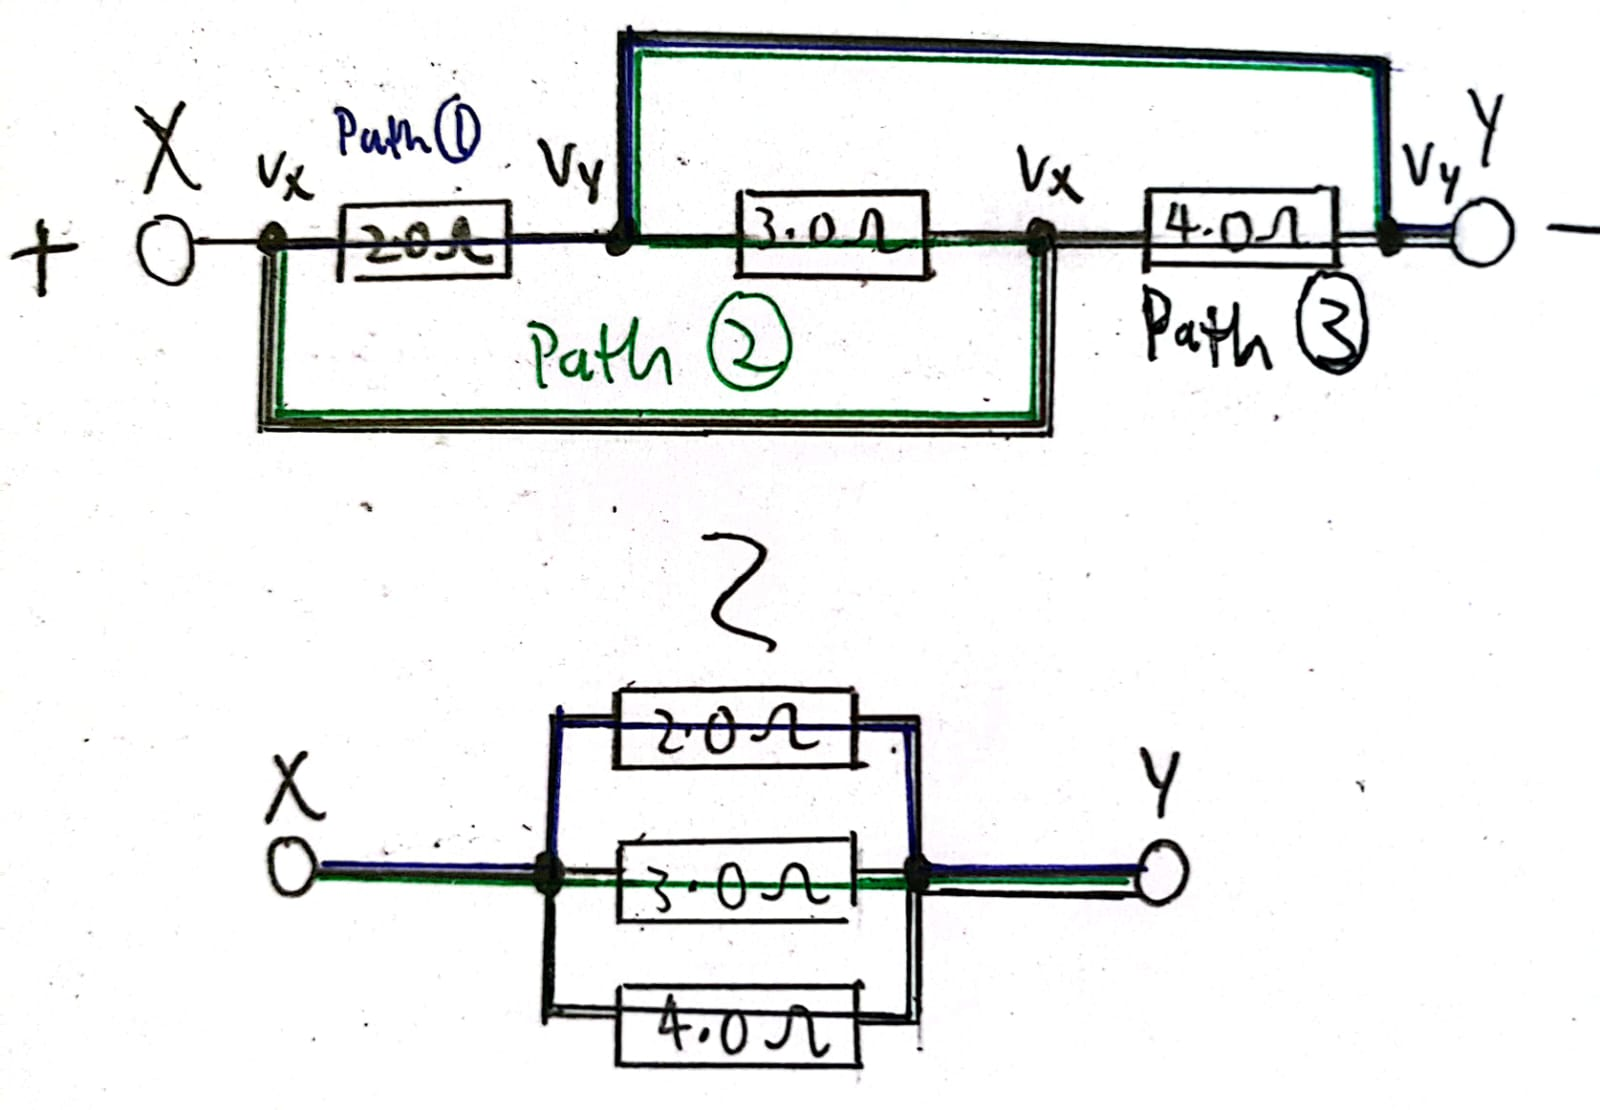
\includegraphics[width=\textwidth]{../images/DC-Circuits-Resistors.jpg}
            \caption{}
            \label{}
        \end{subfigure}\hfill
        \begin{subfigure}{0.45\textwidth}
            \centering
            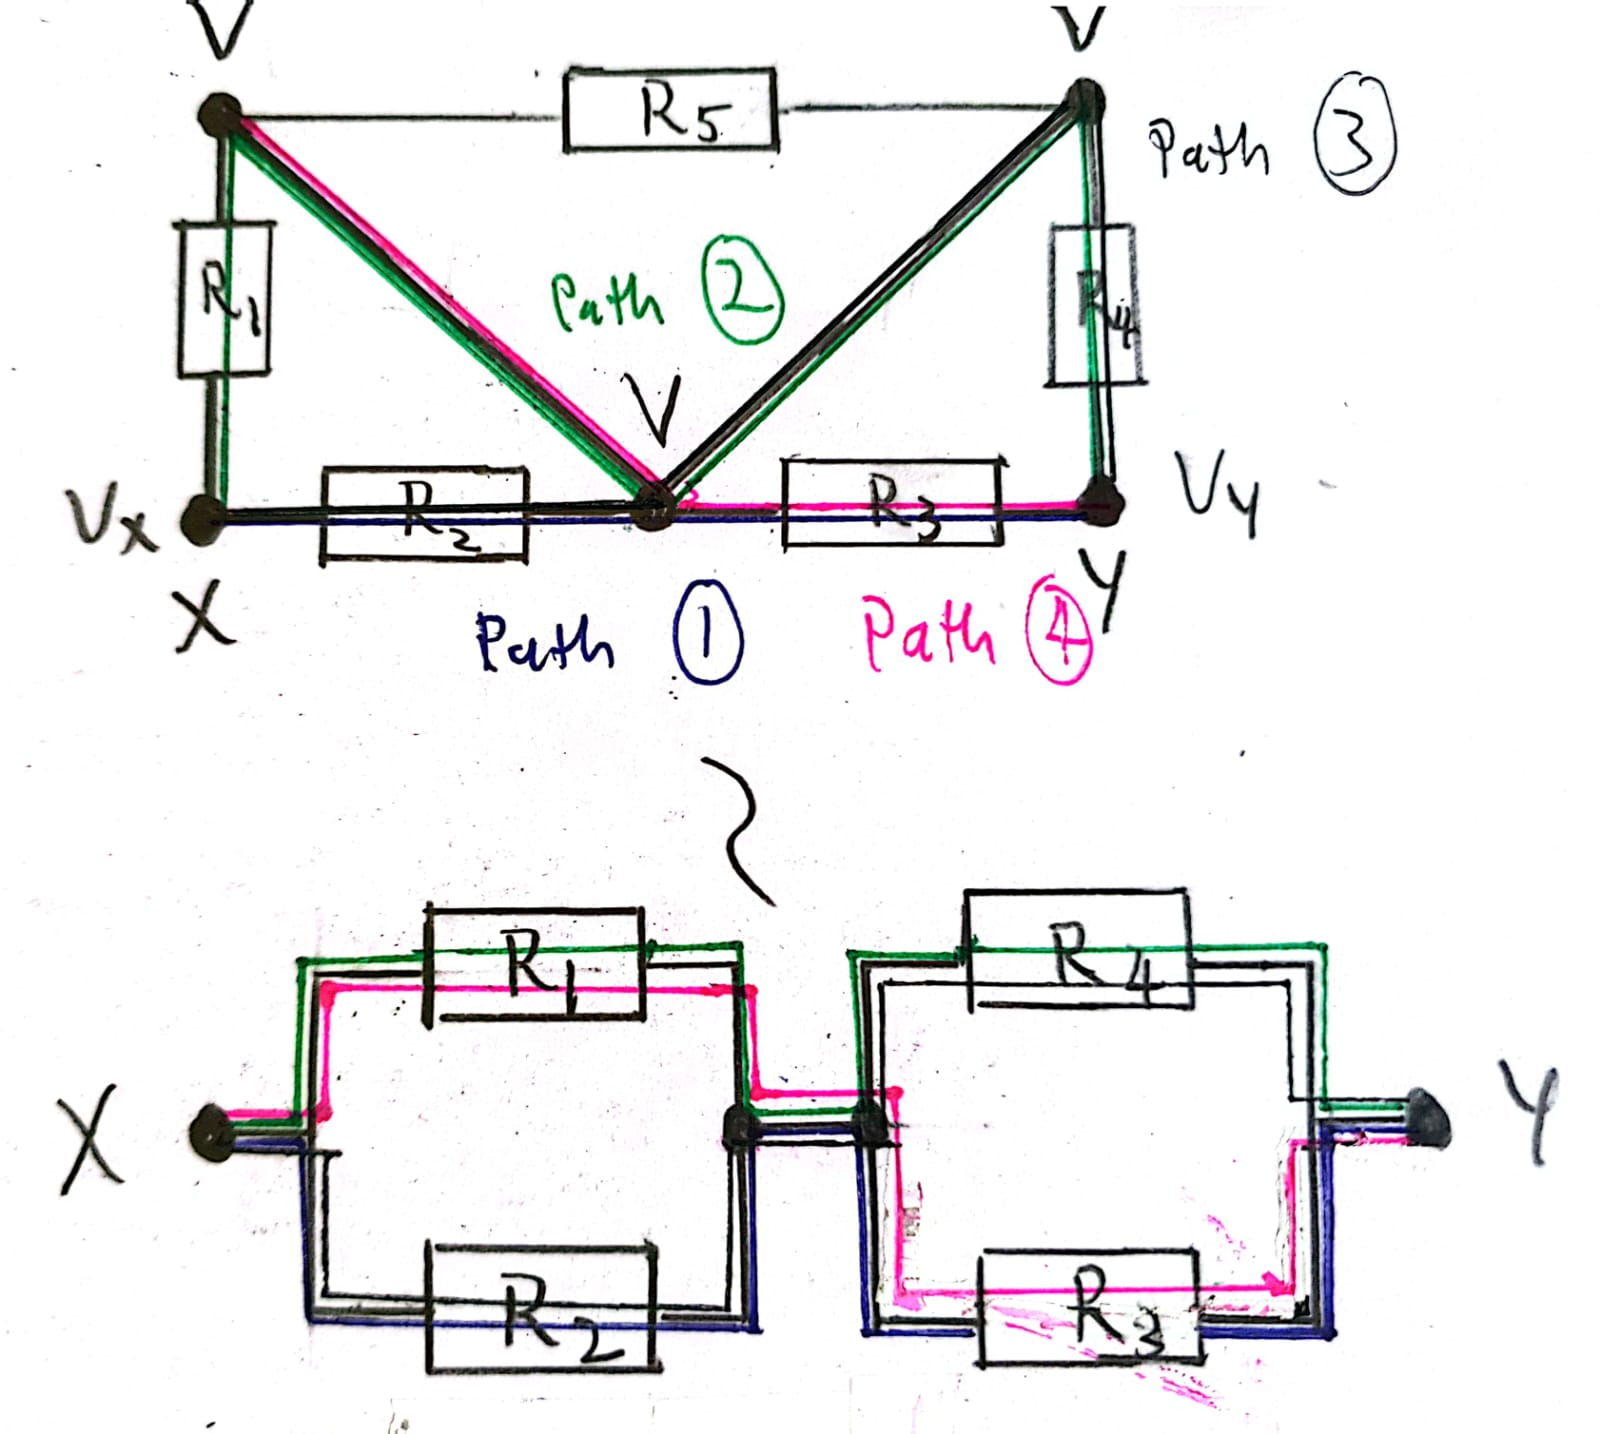
\includegraphics[width=\textwidth]{../images/DC-Circuits-Resistors2.jpg}
            \caption{}
            \label{}
        \end{subfigure}
        \caption{\ref{Me} Some tricky circuits.}
        \label{fig:tricky-circuits}
    \end{figure}
    \item Potentiometer:
    \begin{itemize}
        \item E.m.f. of driver cell is more than that of the unknown cell, \(E\).
        \item The direction of charge flow for the primary and secondary circuits are opposite. i.e. the positive/negative terminals should `point' towards each other.
        \item The potential difference \(V\) across length \(L\) of a resistance wire is directly proportional to \(L\).
        \item Consider the following circuit. When the galvanometer reads zero, the e.m.f. of the unknown cell is \(E_{AJ}\), where 
        \[\frac{E_{\text{AJ}}}{E}=\frac{L_{\text{AJ}}}{L_{\text{AB}}}=\frac{R_{\text{AJ}}}{R_{\text{AB}}}.\]
        \begin{figure}[H]
            \centering
            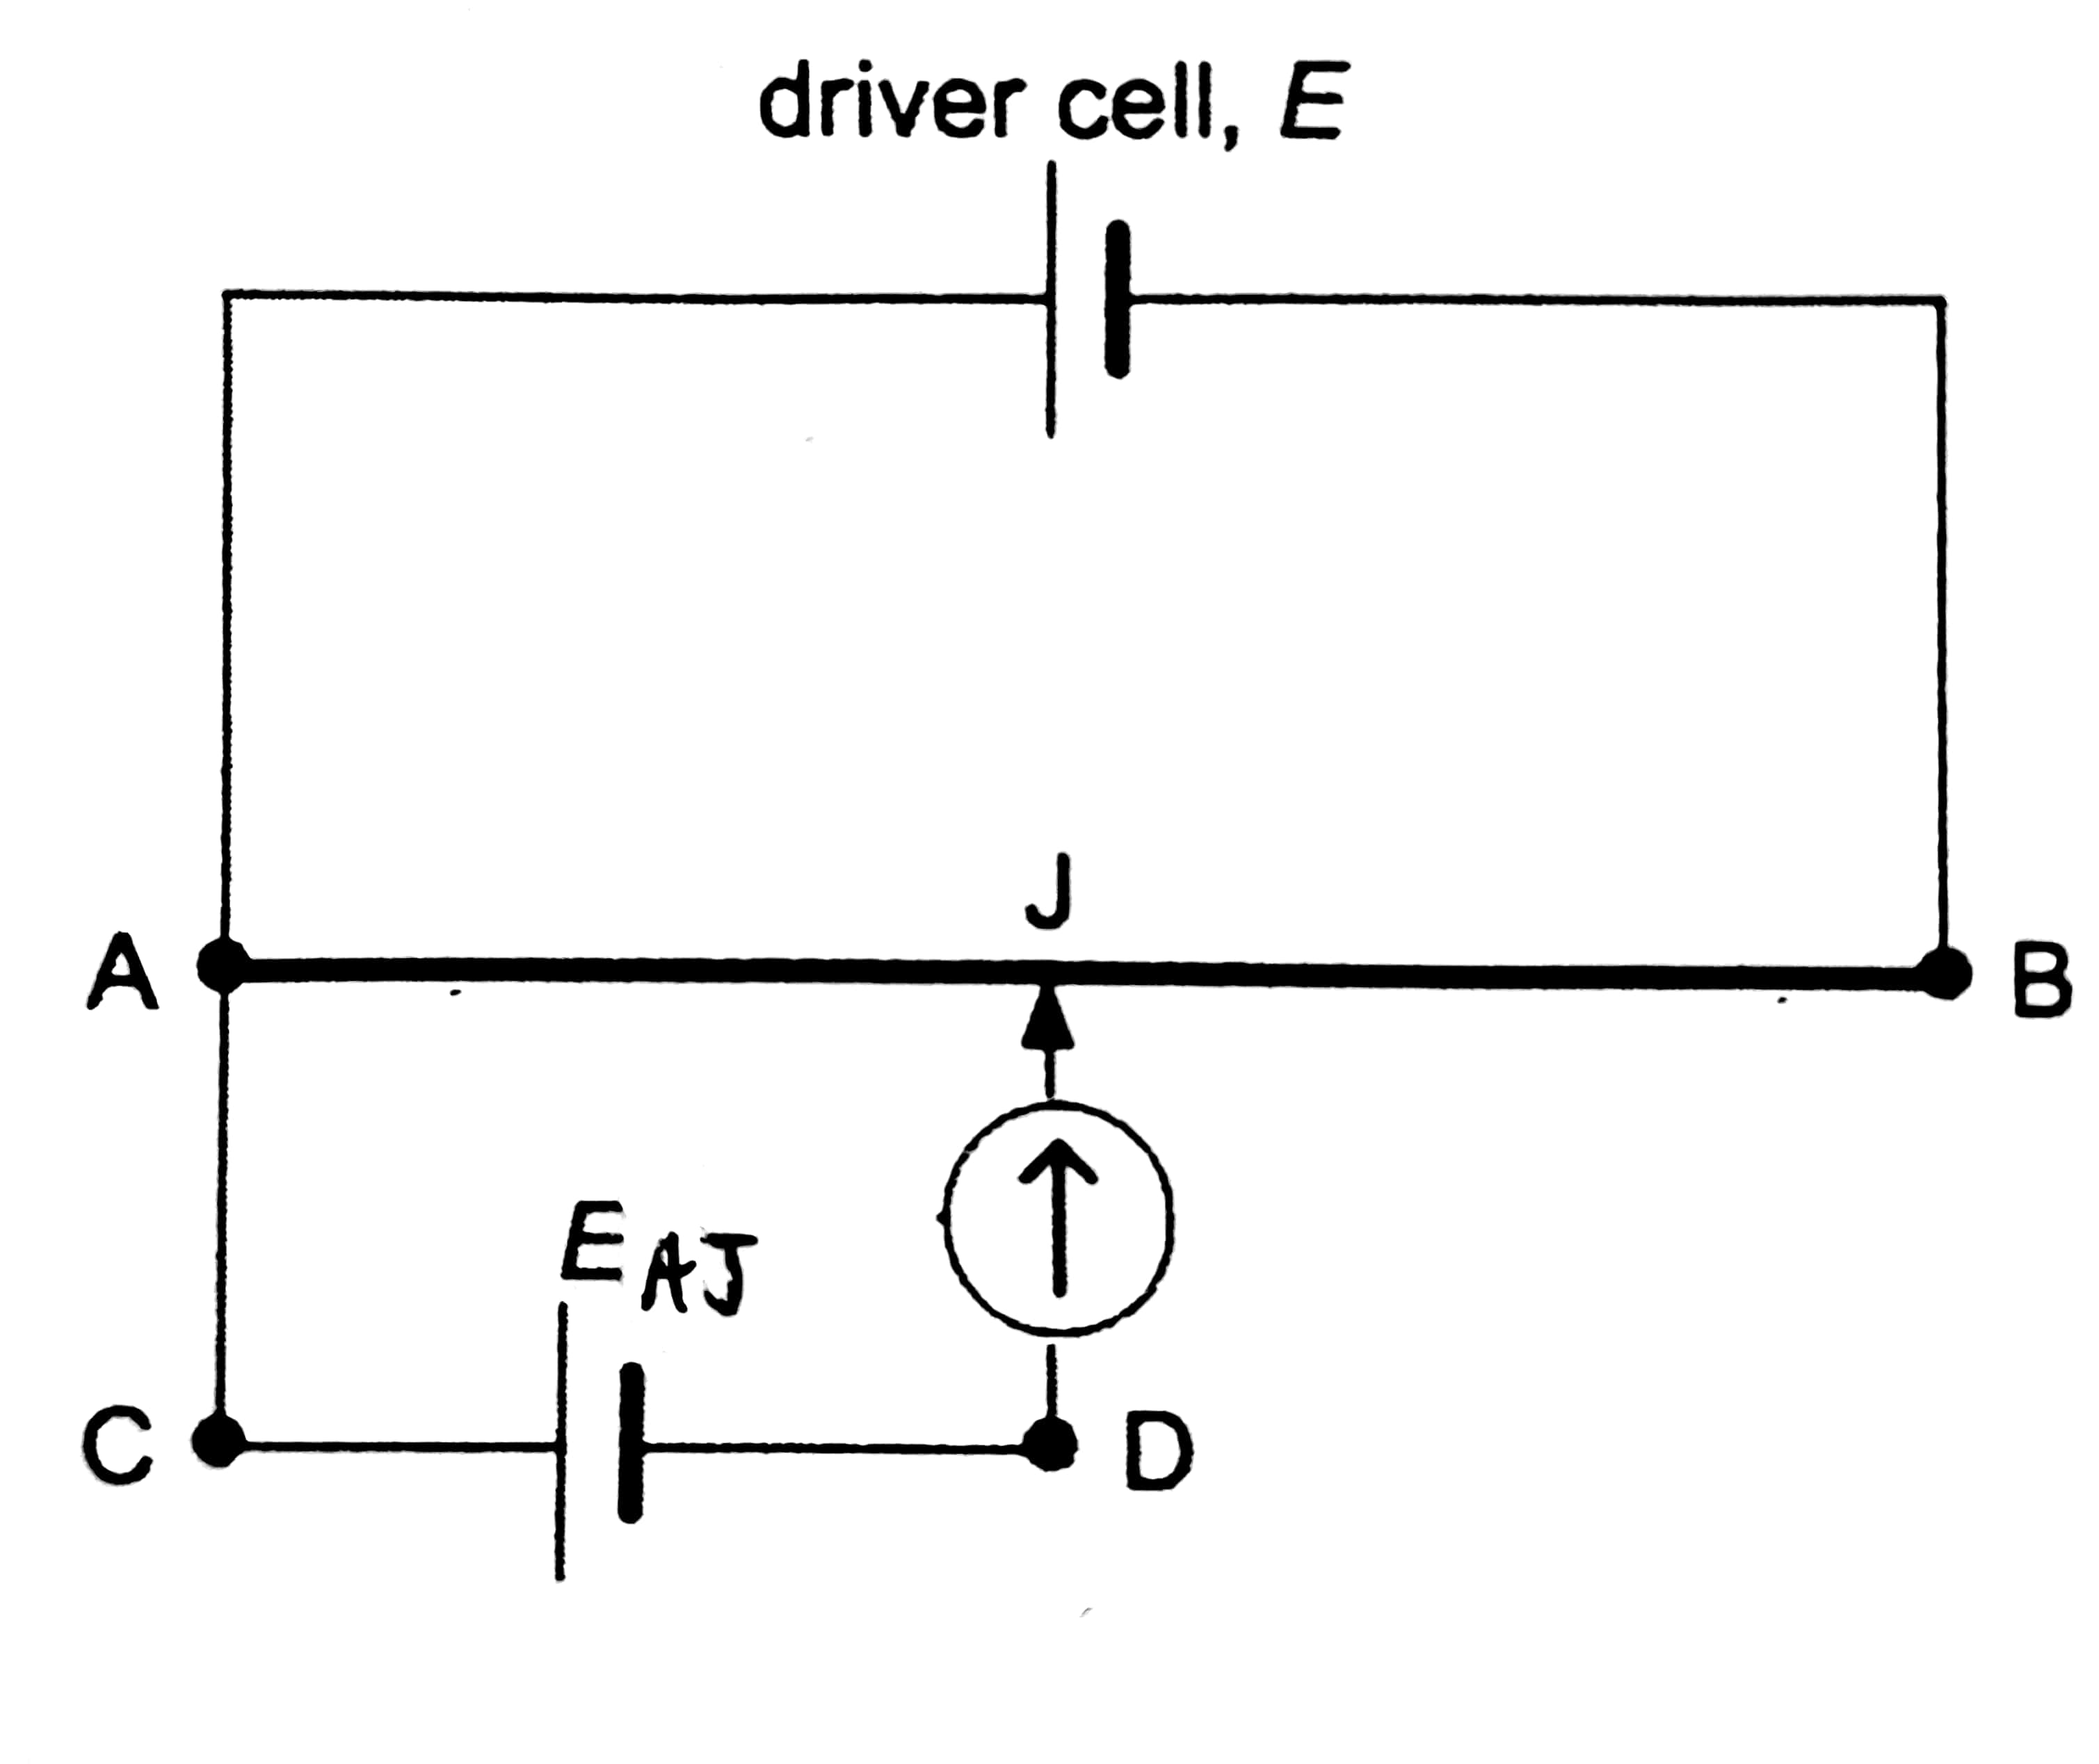
\includegraphics[width=0.4\columnwidth]{../images/DC-Circuits-Potentiometer-1.jpg}
            \caption{\ref{Me} An illustration of a potentiometer.}
            \label{fig:potentiometer}
        \end{figure}
        \item In the circuit below, the internal resistance \(r\) satisfies
        \[\frac{L_{AJ_2}}{L_{AJ_1}}=\frac{R}{R+r}.\]
        \begin{figure}[H]
            \centering
            \begin{subfigure}{0.45\textwidth}
                \centering
                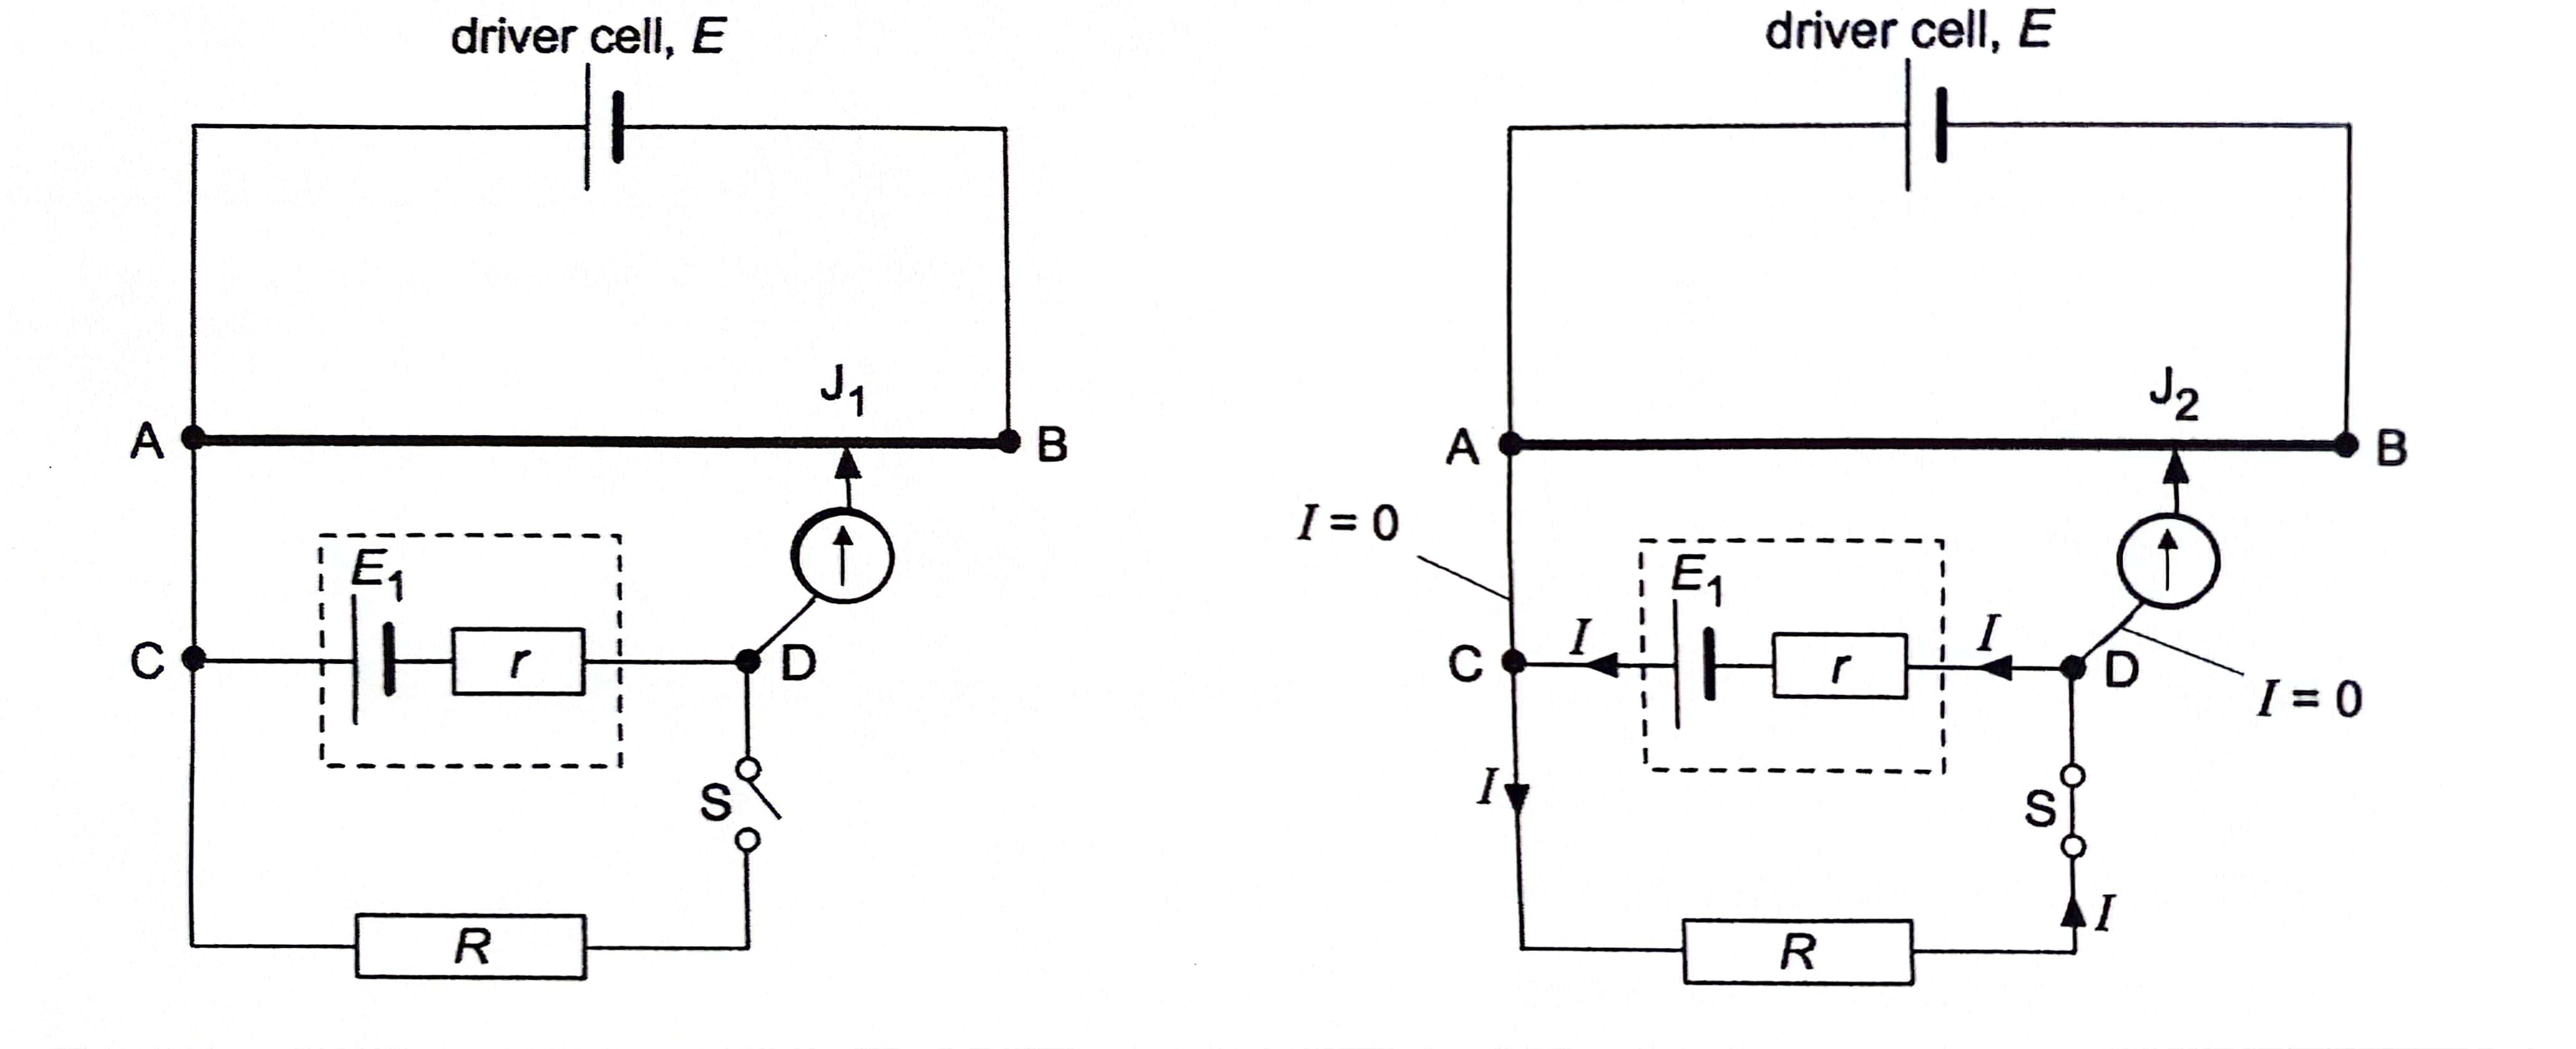
\includegraphics[width=\textwidth]{../images/DC-Circuits-Potentiometer-2.jpg}
                \caption{Open switch.}
                \label{fig:potentiometer-open-switch}
            \end{subfigure}\hfill
            \begin{subfigure}{0.45\textwidth}
                \centering
                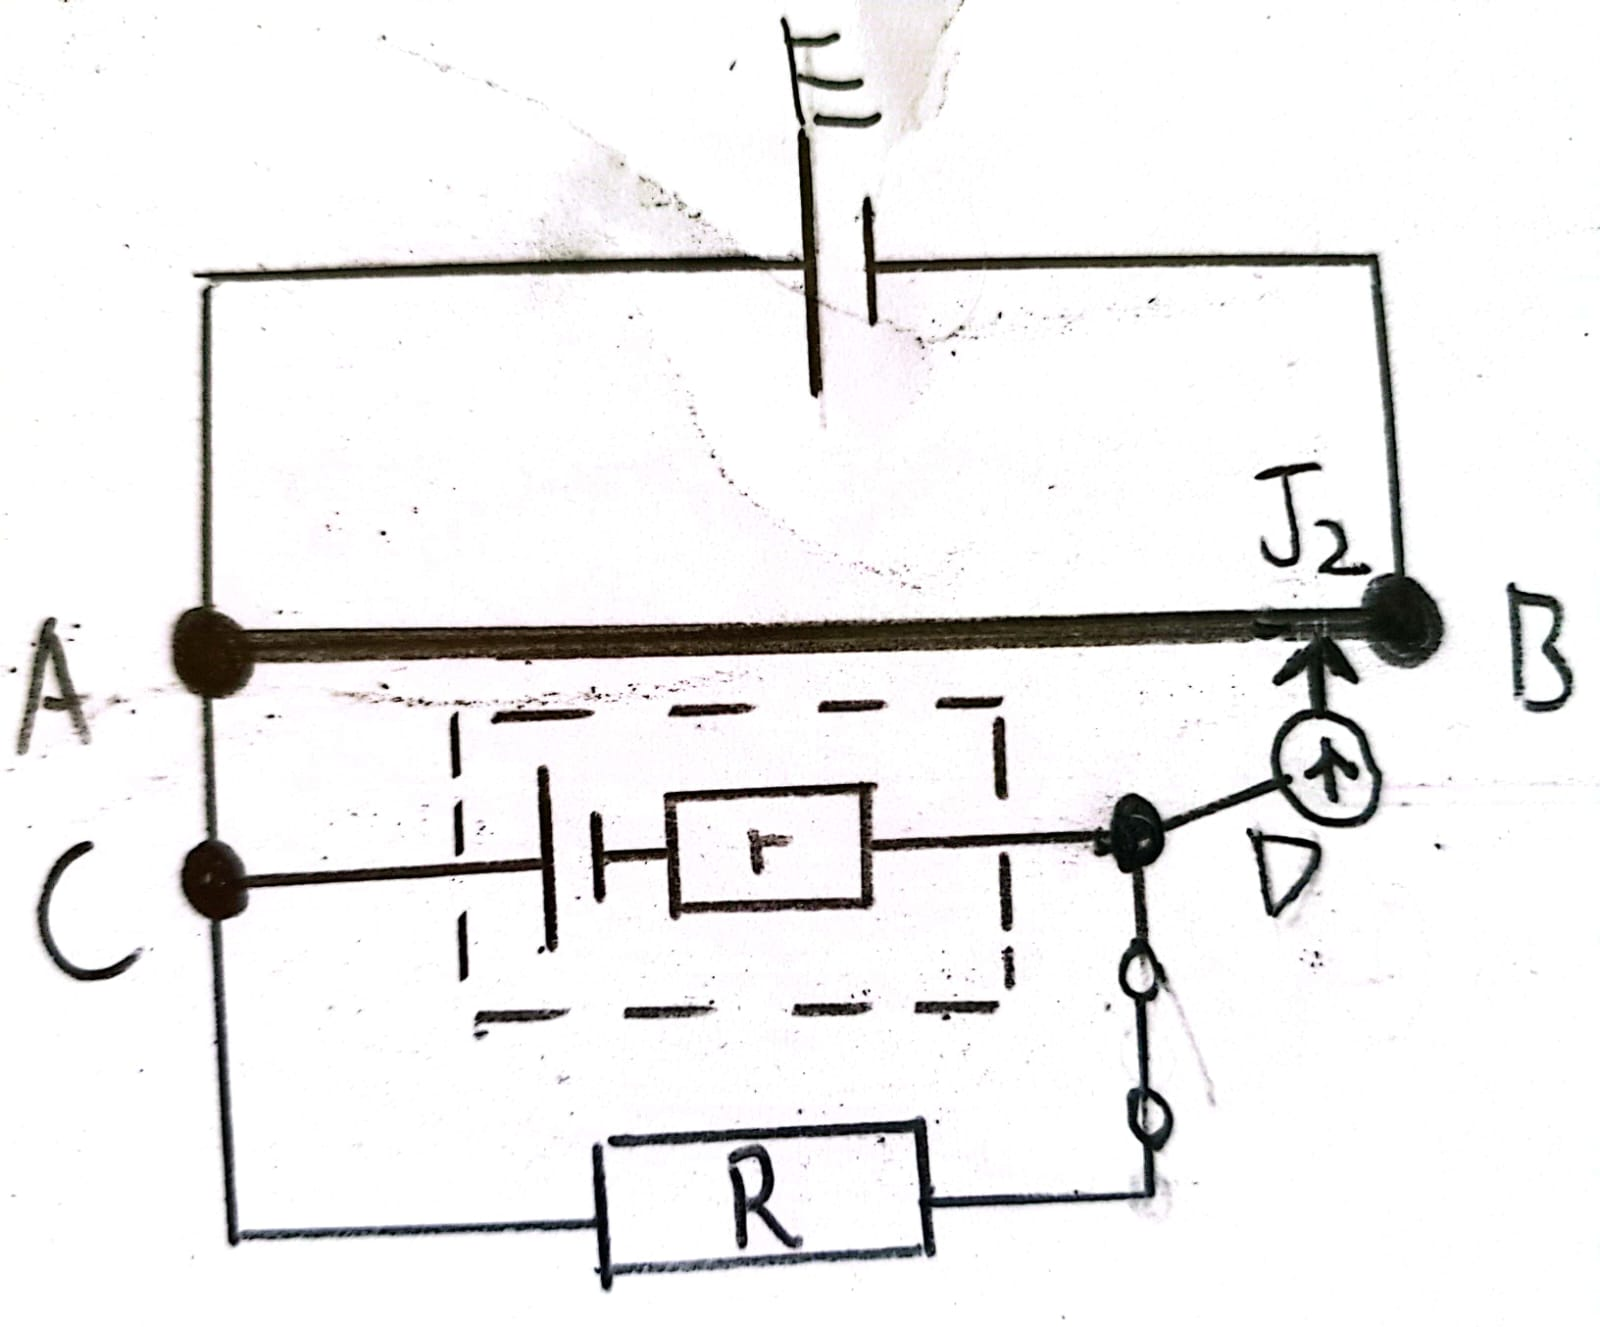
\includegraphics[width=\textwidth]{../images/DC-Circuits-Potentiometer-2.2.jpg}
                \caption{Closed switch.}
                \label{fig:potentiometer-closed-switch}
            \end{subfigure}
            \caption{\ref{Me} A potentiometer with a resistor parallel to the secondary circuit.}
            \label{fig:potentiometer-parallel-resistor}
        \end{figure}
        For the diagram to the left, why \(V_{CD}=V_{AJ_1}\) is easily seen from the diagram below.
        \begin{center}
            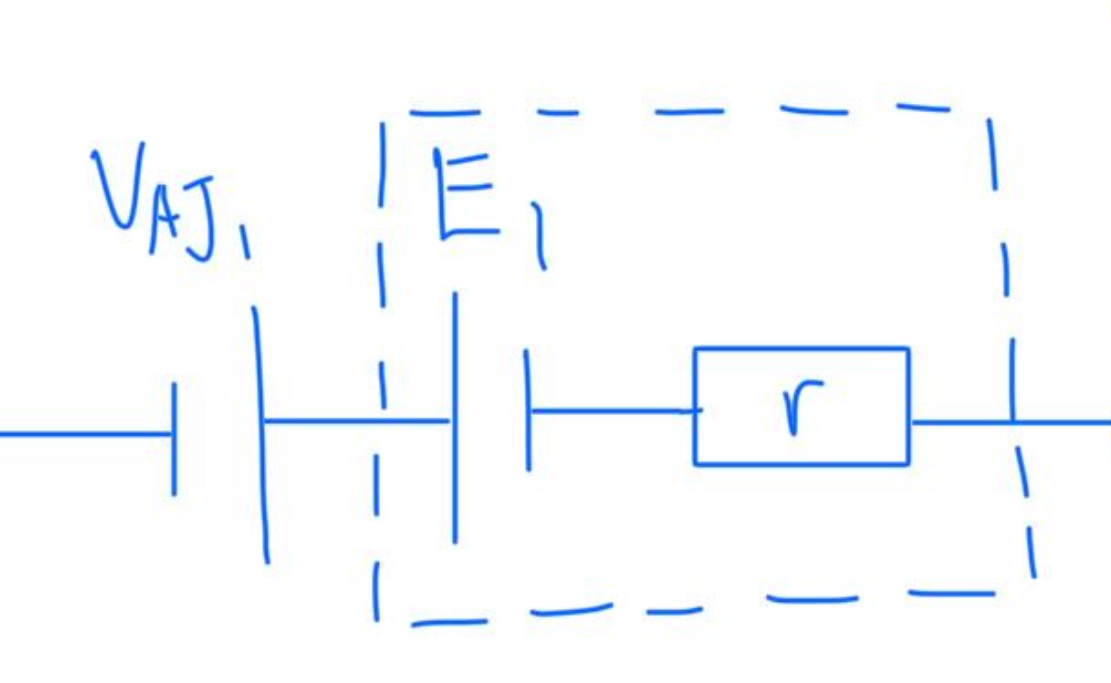
\includegraphics[width=0.3\columnwidth]{../images/D.C.-Voltage-Cancelling-Each-Other.png}
            \captionsetup{type=figure}
            \caption[figure]{\ref{Me} Part CD of the circuit.}
        \end{center}
    \end{itemize}
\end{itemize}